
%
%  $Description: Author guidelines and sample document in LaTeX 2.09$
%
%  $Author: ienne $
%  $Date: 1995/09/15 15:20:59 $
%  $Revision: 1.4 $
%

\documentclass[10pt,twocolumn,ieeetran]{article}
\usepackage{latex8}



\usepackage{picture}
\usepackage{listings}
\usepackage{tikz}
\usepackage{verbatim}
\usepackage{pgf-pie}
\usetikzlibrary{shapes,decorations}
\usetikzlibrary{decorations.text}
%\usepackage{marvosym}
\usepackage{amssymb}
\usepackage{fancyheadings}

\usepackage{pgfplots}
%\usetikzlibrary{chain}

\usetikzlibrary{shapes.callouts}
\usepackage{theorem}
\usetikzlibrary{decorations.pathmorphing,backgrounds,fit}

\usetikzlibrary{arrows,shapes.misc,chains,positioning,scopes,calc,through,backgrounds,fadings} 

\usetikzlibrary{mindmap,trees}

\usepackage{pgfplots}
\usetikzlibrary{patterns}
\usetikzlibrary{calc,3d}


\usetikzlibrary{shapes,snakes}
\usepgflibrary{decorations.markings}

%\documentclass{book}

\usetikzlibrary{calendar} % LATEX and plain TEX

%\usepackage{times}

%\documentstyle[times,art10,twocolumn,latex8]{article}
\usepackage{tikz}

%-------------------------------------------------------------------------
% take the % away on next line to produce the final camera-ready version
\pagestyle{empty}

\usepackage{tikz}

\tikzset{ 
  nonterminal/.style={ 
    % The shape: 
    rectangle, 
    % The size: 
    minimum size=6mm, 
    % The border: 
    very thick,           
    draw=red!50!black!50, % 50% red and 50% black, % and that mixed with 50% white 
    % The filling: 
    top color=white,               % a shading that is white at the top... 
    bottom color=red!50!black!20, % and something else at the bottom 
    % Font 
    font=\itshape                 
  }, 
  terminal/.style={ 
    % The shape: 
    rounded rectangle, 
    minimum size=6mm, 
    % The rest 
    very thick,draw=black!50, 
    top color=white,bottom color=black!20, 
    font=\ttfamily}, 
  skip loop/.style={to path={-- ++(0,#1) -| (\tikztotarget)}} 
} 

\newcommand{\marginlabel}[1]{\mbox{}\marginpar{\raggedleft\hspace{0pt}#1}}
\tikzstyle{every node}=[font=\small, text centered, node distance=1.5cm] 
\tikzstyle{decision} = [diamond, draw, fill=red!20, 
    text width=4.5em, text badly centered, node distance=2cm,minimum height=0.6em, inner sep=0pt]
\tikzstyle{block} = [rectangle, draw, fill=blue!20, 
    text width=7em, text centered, rounded corners,  minimum height=0.5em]
\tikzstyle{line} = [draw, -latex']
\tikzstyle{cloud} = [draw, ellipse,fill=red!20, node distance=3cm,
    minimum height=2em]

\newenvironment{matrixtable}[4]{%
  \begin{tikzpicture}[matrix of nodes/.style={
    execute at begin cell=\node\bgroup\strut,
    execute at end cell=\egroup;}]
  \matrix (m) [matrix of nodes,top color=violet!40,
    bottom color=violet!80,draw=white,
    nodes={draw,top color=violet!35,bottom color=violet!45,
    draw,inner sep=2pt,minimum height=3.1ex},
    column sep=0.2ex,row sep=0.2ex,inner sep=0.5ex,
    rounded corners,column 1/.style={minimum width=#1},
    column 2/.style={minimum width=#2},
    column 3/.style={minimum width=#3},
    column 4/.style={minimum width=#4}]}%
{;\end{tikzpicture}}

\tikzset{ 
  nonterminal/.style={ 
    % The shape: 
    rectangle, 
    % The size: 
    minimum size=6mm, 
    % The border: 
    very thick,           
    draw=red!50!black!50, % 50% red and 50% black, % and that mixed with 50% white 
    % The filling: 
    top color=white,               % a shading that is white at the top... 
    bottom color=red!50!black!20, % and something else at the bottom 
    % Font 
    font=\itshape                 
  }, 
  nontermina2/.style={ 
    % The shape: 
    rectangle, 
    % The size: 
    minimum size=6mm, 
    % The border: 
    dotted,           
    draw=red!50!black!50, % 50% red and 50% black, % and that mixed with 50% white 
    % The filling: 
    top color=red,               % a shading that is white at the top... 
    bottom color=red!50!black!20, % and something else at the bottom 
    % Font 
    font=\itshape                 
  }, 
  terminal/.style={ 
    % The shape: 
    rounded rectangle, 
    minimum size=6mm, 
    % The rest 
    very thick,draw=black!50, 
    top color=white,bottom color=black!20, 
    font=\ttfamily}, 
  skip loop/.style={to path={-- ++(0,#1) -| (\tikztotarget)}} 
} 

%-------------------------------------------------------------------------

%-------------------------------------------------------------------------


\title{Towards a Social Interaction-based Cognition Model: An Analysis of Spatial Data Infrastructure}

\author{Luis Reynoso, Eduardo Grosclaude, Laura S\' anchez \\
Facultad de Inform\' atica\\ {\it Universidad del Comahue, Argentina} \\
{\it Buenos Aires 1400 (8300) Neuqu\'en}\\ \{Luis.Reynoso, Eduardo.Grosclaude,  Laura.Sanchez\}@fai.uncoma.edu.ar\\
% For a paper whose authors are all at the same institution,
% omit the following lines up until the closing ``}''.
% Additional authors and addresses can be added with ``\and'',
% just like the second author.
\and
Mabel \' Alvarez\\
{\it Universidad de la Patagonia San Juan Bosco, Argentina}\\
{\it Belgrano y Rawson (9100) Trelew, Chubut}\\
mablop@speedy.com.ar\\
}


% Java Code: 
\lstdefinelanguage{Java}{morekeywords={print,while,def,for,in,range,public,double,static,void,class,method,int,if,else,new,main,boolean,type,strings,char,package,private,null},
keywordstyle=\color{blue}\bfseries\sf,sensitive=false,morecomment=[l]{//},morecomment=[s]{/*}{*/},morestring=[b]",}
\lstset{language=Java, basicstyle=\normalsize, numbers=none, numberstyle=\bf, tabsize=2}
\definecolor{gg}{rgb}{0,90,0} % definicion rgb para un color
\definecolor{comentarios}{rgb}{150,150,150} 
\lstset{morecomment=[l][\color{gray}\bfseries\sf]{//}}
\lstset{stringstyle=\color{orange}\bfseries\sf}
\lstset{morestring=[b][\color{orange}\bfseries\sf]{"}{"}
}
% fin Java Code


\begin{document}
\maketitle
\thispagestyle{empty}




\begin{abstract}
Distributed cognition is a psychological theory which assumes that knowledge lies not only within the individual but also in the individual's social and physical environment. Today, we tend to achieve cognitive results by means of a sequence of complex and subtly interwoven interactions, using  technological devices, and with the help of other, more knowledgeable people. As dwellers of a new century, we are agents of a novel technological assembly where knowledge is socially produced, and nurtured by the various sources of many communities of practice (CoP). In this paper we propose a social interaction-based cognition model which applies distributed cognition and interoperability between different actors of CoP in web environment. The core components of the model are: Authenticity and Cohesion, Assemblage and Shared Meanings. We also present the main findings of qualitative research in a case of study to Spatial Data Infraestructure (SDI) and CoP around this technological assemblies. 
%Requeriments to built an SDI includes: to share a common representation of the space according to different aspects: administrative, technical, semantic interoperability, to work in CP and to apply distributed cognitions and conceptions. 
% the social coordinations about their space
% http://tecfa.unige.ch/tecfa/publicat/dil-papers-2/

\end{abstract}

{\bf Keywords:} Social Interaction. Distributed Cognition. Communities of Practice. Interoperability. 


%-------------------------------------------------------------------------
\Section{INTRODUCTION}

SURROUND vs ENVIRONMENT\\
PERSON vs INDIVIDUAL

%Cognitive theories show a strong vias toward an analysis of the individual while thinking and learning.
Studies have traditionally considered cognitive processes \cite {Wang2005} and development as something possessed by individuals and residing in their heads. Accordingly, cognitive models have been reduced to the process being carried on by an individual.  
However, thinking and learning often involve relinquishing some higher-order knowledge and executive functions to the environment in worthwhile ways. 
From a distributed-cognition-based perspective, 
the person and its surround are taken into account as a single system 
in order to analyze  thinking and learning contexts and processes. 
As for the person's surround, both social and technological factors need to be considered. Both undoubtedly contribute to cognitive development; they are more than external sources of stimulation.

The social development theory by Vygotsky \cite{Wertsch} constitutes an important framework 
dealing with the social surround of the learning process. Vygotsky's theory involves an individual, with the help of \emph{more knowledgeable others} (\emph{MKO} in Vygotsky's theory), in a \emph{zone of proximal development (ZDP)} environment. Our reasoning can be expressed in this way: without help from others, many of our ablest learning experiences, such as those resulting from interaction between the individual and \emph{MKO},  could not be performed. Distributed cognition describes the cognitive aspects which are triggered between these individuals involved in the process, with the consideration of technological resources and environment.

The theory of distributed cognition \cite{Salomon} does not oppose to existing cognitive theories of the isolated individual. It rather encompasses those theories within a wider model where cognitive aspects are not just produced by an individual but also by the interaction among subjects, and between subjects and their environment.

We believe whether anything remains to study in existing cognitive models is the topic of interaction. The study of social interaction and cognitive interaction will contribute to understand social cognition and knowledge of humanity \cite{Denny} that endures and grows beyond the life of an individual.

In that study, the application of distributed cognition could be complemented with communities of practice (CP) \cite{Wenger} and social networks (SN) \cite{Kadushin} \cite{Santos}\cite{Watts} theories. When we work in a social network, as well as in CP, we need to think ourselves as an interwoven chain of nodes that interacts between each other. A social network is a social structure made up of social actors (nodes), such as individual, groups or organizations \cite{Wasserman}, \cite{Jamali}. Communities are presents in organizations as in our ordinary life, they are a facet of social networks.

%  such as  IDERA in Argentina, INDE in Brasil, IDEE in Spain, European SDI INSPIRE, etc.
We focus on interoperability of actors within social and technological environment' interactions, as well as on analizing which roles are performed by actors in these contexts. We show the findings of a qualitative 
research we perform with communities of practice around Spatial Data Infraestructure (SDI). SDI had emerged
as a technological solution of this century to manage and analysis the space (land and water). The technological assemblies of organizations within a SDI had evolved and improved in several countries, at
different scales (local, national, regional). SDI requires that each organization participating in building the infraestructure, contribute providing its own space' information (or spacial' hability) within a common framework. Space information which is interchanged share a common technology to allow that the space can be visualized, analyzed and managed accordingly. To get sucha a infraestructure (SDI), social, cultural \cite{Nisbett} and cognitive changes should be produced within intertwined commmunities.

%To address a study of distributed cognition will give us more elements to understand the collective knowledge that remains in the time between communities, regions and the global society. Knowledge that remains through the interaction of oral society, after the legal society and this time with other technological items.


           
The paper is organised as follows. Section 2 introduces the distributed cognition theory. 
Section 3 provides an overview of communities of practice. Section 4 describes the interoperability' hability. Section 5 presents a Y-model of the Social Interaction-based Cognition. 
Section 6 details a case study of communities of practice and interoperability of SDI. 
Section 7 goes on to describe conclusions and future work.
                                       
                                                     
\Section{DISTRIBUTED COGNITION}

This theory was originally developed in the mid-1980s by Edwin Hutchins. Using insights from sociology, cognitive science, and the psychology of Vygotsky (cf. cultural-historical psychology) it emphasizes the social aspects of cognition. The theory provides a more balanced theoretical treatment of problem solving in real work situations, and to supply a new framework for cognitive science generally.
Distributed cognition has been proposed as a new foundation for human-computer interaction \cite{Hollan}. 


The unit of analysis is different from previous cognitions studies. The theory of distributed cognition employs a variable unit of analysis.  Traditional cognitive theory takes the individual person as the proper unit of analysis.  On this traditional view, cognitive processes are internal processes.  The social, technological and cultural context is thus often left out of the analysis. In contrast, the theory of distributed cognition makes of the individual and its socio-cultural context a larger cognitive system, one that is to be analyzed in a broadly traditional way, as a computational system. 
Enlarging the unit of analysis in this way has the benefit that representations internal to the system are now external representations with respect to the individual agents that use and make use of them. 
So, distributed cognitions is conceived as a system that entails both person and surround \cite{Salomon}.

Distributed cognition can be considered aligned with Vygotsky and Cole: (1) Vygotsky cultural-historical theory \cite{Wertsch}, a theory that situates individual cognitions within, rather than just interacting with, social and cultural contexts of interaction and activities \cite{Salomon}; (2) Cole who had pointed out \cite{Cole} that the proper unit of psychological analysis should be the joint socially mediated activity in a cultural context.

%The first and most fundamental rule according Durkheim \cite{Durkheim} is: Consider social facts as things.
%sociology of the technology \cite{Thomas}

Within distributed cognition, Perkins \cite{Perkins}, \cite{Perkins2} introduces a learning model in which he proposes to take as his unit of analysis not the learner without resources in his or her surround -the person-solo- but the {\it person-plus} surround, or person-plus for short. People employ the surround to support, share and undertake outright aspects of cognitive processing. That is the perspective taken by the person-plus on thinking and learning contexts, to treat the person plus surround as one system.
He also introduces the concept of {\it equivalent access hypothesis}, which distinguishes four factors: the kind of knowledge, the way it is represented, how readily it is retrieved, and how it is constructed \cite{Salomon}.

The existing literature includes many examples of distributed cognition. They are diverse with different complexity. Simple examples involve problem-solving using pencil and paper or computers, to more complex methaphors in the context o navigation a navy vessel, or crewing a plane \cite{Hutchins95}. 
%counting as part of the thinking what gets done or partly done in the surround (perkins)


We think that the study of distributed cognition may alleviates cognitive drawbacks of learning designs based on traditional cognitive models: 

\begin{itemize}

\item People often fail to apply knowledge and skills learned in one context to other situations \cite{Perkins} (cognitive transfer). Distributed cognition emphasize collaborative learning, learning by practice and learning within communities of practice.

\item People often fail to decontextualize \footnote{Decontextualizing \cite{Wertsch} is the handling of information in a way that either disconnects other information or backgrounds it \cite{Denny}, it is produced when the meaning of the signs is becoming less dependent on the spatial and temporal context in which they are used. For example, when we obtain (to induce) a general rule for a set of observed facts we abstract/produce a common structure behind the observed cases, so changing of propositional levels is applied.}: Cognitive decontextualization is required cognitive activity previous to apply cognitive transfer.  

\item People often fail to solve problems applying mediators instruments (such as technological resources).
Cognitive distribution considers that thinking and learning often involve ceding some higher and executive function to the surround in worthwhile ways. Commonly, this ceding includes the use of technological devices and resourse which should take into account. Distributed cognition analyze the interaction between subject and objects.   
\end{itemize}



%Social Networks \cite{Santos}, \cite{Watts}.





\Section{COMMUNITIES OF PRACTICE}

Learning is not an activity that can be carried out in isolation, we learn from other people, either from the culturally produced artifacts that provide mediators elements \cite{Wells}. Wells \cite{Wells} argues that to understand learning we need to understand how a individual, as a member of a community, applies and produce representations in the collaborative effort to transform their shared world.

% conocer no es una actividad que se pueda llevar a cabo en aislamiento, aprendemos bien de otras personas o bien de los artefactos culturalmente producidos que proporcionan los elementos mediadores. (Wells 2001)

%as pointed out by Cole \cite{Salomon}

Wenger \cite{Wenger} argues that the primary unit of analysis (in sociological studies) is neither the individual nor social institutions but rather the informal communities of practice that people form as they purse shared enterprises over time \cite{Wenger}. The author emphasize that engagement in social practice is the fundamental process by which we learn and so become who we are. Three processes for individual and group identity formation are identified in communities of practice, as the key elements for individual membership identity as well as for developing community identity: (1) mutual engagement, (2) joint enterprise, and
(3) shared repertoire.


Learning takes place during active participation in a social group, which not only allows the individual to become a member, but also provides the elements for that individual to construct an identity through these communities. Individual identity, as well as social identity, affects the perception of the group and its common repertoire. Perception in consequence affects cognition and influences in their tasks.

%Las comunidades de practicas estan compuestas por actores que pueden ser organismos.-
\Section{INTEROPERABILITY}

A property of distributed cognition is its constituents be interchangable. When we analize distributed
cognition in web invironment the access to resources and between actors is crucial. Distributed cognition
is not conceived without communication neither without hability of its members to communicate.

Interoperability is the ability of making systems and organizations to work together (inter-operate). People (or organizations) working within an interoperable environment should develop a capacity or hability to interchange (and retrieve) knowledge, as well as to use the interchanged knowledge and to build new one upon them. 
While the term, interoperability, was initially defined for information technology or systems engineering services to allow for information exchange, a more broad definition takes into account social, political, and organizational factors that impact system to system performance.

The three dimensions of interoperability include:

\begin{itemize}

\item Technical interoperability: refers to those technical issues to ensure that the technological components of information systems of participating actors are prepared to work together. Therefore  it lets provide common mechanisms for transferring data and invocation of functions, transparent to networks substratum and information systems (applicable to multi-platform, multi-language systems). Among other questions, it refers to interfaces, interconnection services, data integration, middleware, data presentation and exchange, accessibility, open systems and secure systems. It  comprises the use of technology to manage information structure, the structure of services, semantics of information, and semantics of web services \cite{Moreno}. The technical dimension of interoperability allows us to analyze an economic perspective of  interoperation between actors. When considering the different roles that the actors can take in terms of consumer / producer, or supply / demand information (even other roles of the model RM-ODP) we can have a clear view of flow and traffic information .

\item Semantic interoperability: It deals with the meaning in the use of data and information and, in particular, ensures that the precise meaning of exchanged information can be understood by any application. The information must be interpreted in an univocal manner. Actors usually handle own definitions of information, which often introduces a disadvantage for the exchange of information. The information that is unequivocally performed is easier to be exchanged and interpreted, ensuring an adequate flow of information \cite{Moreno}.
In this matter it is necessary to comply with a formal mechanism to define common elements. This mechanism should ensure quality, must be accepted and respected. Formal documentation that defines the data  must  be formally managed, allowing  the actors to maintain reliability in them.  On the other hand,they should be disseminated by the mass media, being  available to every actor. Additionally, if the definitions are adapted to new requirements,  the compatibility backwards must be guaranteed  with previous definitions. Some of the tools available are classification systems, thesaurus, metadata, and ontologies. 
Organisational interoperability: This deals with the definition: (1) business goals, (2) modeling business processes, and (3) facilitate the collaboration of administrations that wish to exchange information by maintaining different structures and internal business processes of government \cite{Moreno}.

\item Organisational interoperability ensures alignment of administrative procedures involved in the provision of e-government services. In practice this means  defining, collaboratively, the why and when  of  the trading of information, rules and regulations that ensure safety in such trade or plans that will guide the implementation of the initiatives.
It is also responsible for analyzing the gaps in provision of information and even overlaps of responsibilities in information and processes \cite{Moreno}. In other words  it attends  the analysis of boundaries, scope and information links and processes between actors.
The semantic dimension of information exchanged and its own interpretation is in relation to the perspective of the symbolic space of society. For example, an ontology is the conceptualization of collective concepts and semantic relationships established between them in a particular domain.
This collective conceptualization is itself a symbolic construction which in turn is based on cognitive and individual representations of the domain. Finally, it is important to note that in the field of symbolic space also resides the public sphere and field of action of civil society, and it is from these that modifications to the new social space are made.
It is through the symbolic space that individuals and institutions can demonstrate their agency capacity  \cite{Bandura}. Many times this is an individual agency capacity, but in an interoperable space  it can be developed as a whole (and affects) their immediate environment (proxy agency in the theory of Bandura \cite{Bandura}).


The organizational dimension of interoperability is related to Castells's administrative perspective in \cite{Castells2}. The determination of business processes and competencies of the authenticity of the social partners that interoperate must be analyzed using a formal, legal framework, which allows to formalize what is exchanged, when information is exchanged and what means of security are implemented. These formal frameworks are part of the rules of the institutions. In terms of social capital, a concept that refers to the networks and norms that facilitate collective action \cite{Woolcock} \cite{Uphoff} \cite{Dahal} \cite{Sobel} \cite{Maseda} administrative interoperability relates more to the rules associated with the social capital of a society, and networks to its technical dimension. The determination of gaps or overlapping information, will affect new legislation, which facilitates the adoption of new regulations on the subject.

\end{itemize}

\subsection{Technical Interoperability}
In this section technical interoperability is described in more detail. Technical interoperability describes the system in terms of economic aspects of the relations of production / consumption, supply / demand and the technology used. The regency ISO model for open distributed process (Reference Model for Open Distributed Processing RM-ODP) can be applied and used in the study of these forces of production considered in this aspect of interoperability. Using a distributed model is useful to describe a system regarding to data and services in terms of a number of those involved, whose functions are producers and consumers of data-services, thus contributing to a richer view of the system.

Stakeholders can be categorized according to the roles, which will be briefly described below: Producer (Identified as PRD in Fig. 2): An actor who produces data or services. Provider (Identified as PRV in Fig. 2): An actor who provides data or services to users.

The provider differs from the producer, because an actor can serve as support in providing service without having produced the original data. Political decision maker (Policy Maker, Identified as PM in Fig. 2): An actor that sets economic policies implemented (or needed) by a group of those involved. Broker (Identified as in Fig. 2): An actor who provides assistance to users and providers and assists in negotiating contracts between them and can maintain metadata records on behalf of an owner of a product. Their functions include metadata gathering of producers and suppliers, creating catalogs and providing services based on these catalogs. Value Added Reseller, Identified as VAR in Fig. 2): An actor that adds some feature to an existing product or group of products, and then makes it available as a new product. End User Identified as EU in Fig. 2): An actor who uses the information for a specific purpose, an actor with legitimate interest in the use and consumption of data or services provided by other actors.


\Section{SOCIAL INTERACTION-BASED COGNITON}

The computer science has never been alien to the human component in which it is developed, for example by addressing the study of man-machine interfaces, the elicitation of system requirements, etc. In particular, software engineering itself is an inherently human discipline and its measurement makes it closer to the social sciences than the physical sciences \cite{Morasca},  because the phenomena addressing rely on human behavior and these are not easily controlled.
During the last decades,  many human factors and learning characteristics of those who interact with the software have been taken into account (for example the study of man-machine interface, the study of the correlation between learning styles of users and specific software, etc.) and transcultural and global factors in their development (eg. global software engineering).
Likewise when the task of the government proposes reaching  out to citizens through transparent and accessible mechanisms in e-government,  the efforts in the study of government policies have been moving closer to the social sciences, particularly to the society \cite{Graham}.
For example when implementing e-government applications aimed at citizens having at their disposal the functionality they need \cite{Fountain}, beyond the internal division of the government into distinct units, for example with a unique access in a single window \cite{OECD}, implementing electronic voting, etc.. However, the advent of the Internet and the adoption of social networks, have resignified the study on the formation of opinion and communication in society as an important object of study that serves as input for decision-making by governments and market policies.
In this type of study should be highlighted the growing importance areas that are no longer in the individual or institutional spectrum but in the social approach, eg. Studies on Collective Intelligence \cite{Seragan}, Social Web Applications \cite{Bell}, Social Network Analysis \cite{Tsvetovat} and Computational Sociology. These technologies applied to the design and analysis of social networks may allow a better approach to civil society and the public sphere (eg. this strategy has been used in political campaigns with a strong presence in social networks).Thus, we can argue that the social field is of increasing significance.

\subsection{THE PROPOSED Y-MODEL}

Three dimensions compose the Social Interaction-based Cognition (SIbC): CP, CD and Interoperability. Each of them presents three components as Fig. 1 shown through a Y-model. The model is named the Y-model simply because the dimensions of IbSC are presented in the form of the letter Y. The dimensions's components complement between each other, they are semantically connected.

The outside circle of the Y-model shows the cohesion of Social interaction which is primarily based of technical interoperability' habilities, in establishing ties between actors (dyadic, triadic, etc.) through social nets, in maintaining strong and weak interactions. The actors (individual or organizations) of that social interactions reveal specific roles (authenticity).

\begin{figure}[htpb,scale=0.3]
  \centering
  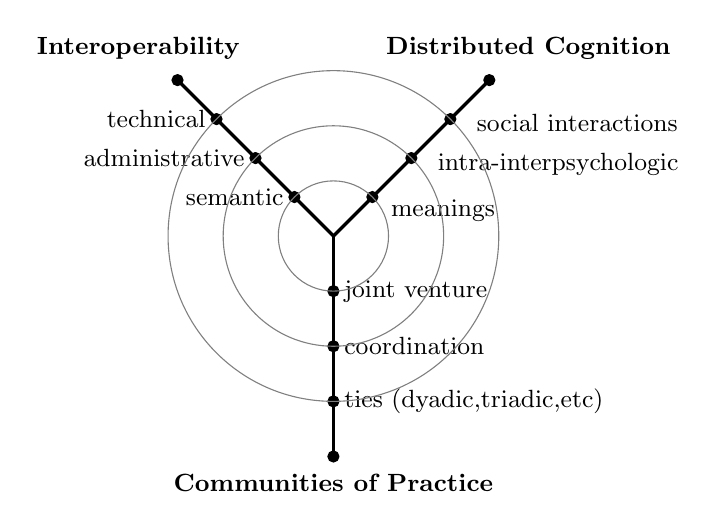
\begin{tikzpicture}[>=stealth',line join=bevel,font=\sffamily,auto,on grid,decoration={markings,mark=at position .5 with \arrow{>}}] 
    %\input{y_chart_common}
    \coordinate (behaviouralNode) at (135:3.5cm);
    \coordinate (structuralNode) at (45:3.5cm);
    \coordinate (physicalNode) at (270:3.5cm);
    \coordinate (originNode) at (0:0cm);

    \node [above=-1.0em] at (behaviouralNode) {\textbf{Interoperability}};
    \node [above=-1.0em] at (structuralNode) {\textbf{Distributed Cognition}};
    \node [below=-1.7em] at (physicalNode) {\textbf{Communities of Practice}};

    \draw[-, very thick] (135:2.8cm) -- (0,0) node[left,pos=0.25]{technical} node[left,pos=0.5]{administrative} node[left,pos=0.75]{semantic};

    \draw[-, very thick] (45:2.8cm) -- (0,0) node[pos=0.15]{social interactions} node[pos=0.4]{intra-interpsychologic} node[pos=0.7]{meanings};

    \draw[-, very thick] (270:2.8cm) -- (0,0) node[right,pos=0.25]{ties (dyadic,triadic,etc)} node[right,pos=0.5]{coordination} node[right,pos=0.75]{joint venture};

    \draw[fill] (barycentric cs:behaviouralNode=0.8,originNode=0.2) circle (2pt);
    \draw[fill] (barycentric cs:behaviouralNode=0.6,originNode=0.4) circle (2pt);
    \draw[fill] (barycentric cs:behaviouralNode=0.4,originNode=0.6) circle (2pt);
    \draw[fill] (barycentric cs:behaviouralNode=0.2,originNode=0.8) circle (2pt);

    \draw[fill] (barycentric cs:structuralNode=0.8,originNode=0.2) circle (2pt);
    \draw[fill] (barycentric cs:structuralNode=0.6,originNode=0.4) circle (2pt);
    \draw[fill] (barycentric cs:structuralNode=0.4,originNode=0.6) circle (2pt);
    \draw[fill] (barycentric cs:structuralNode=0.2,originNode=0.8) circle (2pt);

    \draw[fill] (barycentric cs:physicalNode=0.8,originNode=0.2) circle (2pt);
    \draw[fill] (barycentric cs:physicalNode=0.6,originNode=0.4) circle (2pt);
    \draw[fill] (barycentric cs:physicalNode=0.4,originNode=0.6) circle (2pt);
    \draw[fill] (barycentric cs:physicalNode=0.2,originNode=0.8) circle (2pt);

 %   \draw[black!50] (0,0) circle (4.0cm);
 %   \draw[black!50] (0,0) circle (3.2cm);
    \draw[black!50] (0,0) circle (2.1cm);
    \draw[black!50] (0,0) circle (1.4cm);
    \draw[black!50] (0,0) circle (0.7cm);

  \end{tikzpicture}
  \caption{Y-Model of Int-based Social Cognition} 
  \label{figure:gajski_kuhn_y_chart__levels_of_abstraction}
\end{figure}


The middle circle of the Y-model describes that social interactions is based in confidence and assemblage's links. Assemblage is the product of dialectic process that reside within the intra and interpsychological plane \cite{Wertsch} producing internalization and externalization of actions. Assemblage in social interactions manifiests as summary communication between actors when they are conscious in collaboration tasks avoiding overlaping, or when the 'shared experience' shrinks communication or action. This property is materialized between actors through abstract informal links like confidence, or through objective formal relationships of social contracts (or social procedures).

The inside circle of the Y-model displays the inner core of the model: a joint enterprise is a social construction based in shared meanings between actors, implying a semantic interoperation around a joint repertoire. 


%. Requirement n 1- Commitment The participants recognize the benefits and value of the relationship and are determined to make it work. The level of commitment should progress with time, and the level of responsibility and interaction should increase as the relationship develops. 

%Requirement n 2 - Authenticity Relationships require honesty and candor on both sides. It would be notice if the expressions of care are not sincere, and the relationship will go backwards On the other hand, genuilly expressed appreciation will be quickly perceived and accelerate the evolving relationship. 

%Requirement n 3 - Communication Both parties should feel free to express themselves as they are and known that they will be heard and understood. 

%Governance studies all mechanisms, processes and rules through which ,  economic, political and administrative authority   in an organization, both business and government or the third sector (NGOs) is exerted.  It is a concept that aims to describe a complex systemic transformation that occurs at various levels, from local to global, and among different stakeholders in the public, private and civil sectors. Addressing this concept means tackling social and spatial problems. Social, because it is fundamental both the search for balance and stability of the actors in government of the public and private spheres, as the study of their opinion, perception and participation on the policies and actions of government; and also spatial because it is important to consider the space of configurations adopted by these actors and the adequate management of their own space and resources.  In terms of analyzing each actor we must  pay attention to  which their capacity  / ability is to exchange information and to use the exchanged information, it means, we must consider their level of interoperability.


%social formations are assemblages of other complex configurations, and they in turn play roles in other, more extended configurations.


% !! capacidad de agencia proxy??



\Section{A CASE STUDY: SDI}
In this century, land management's organizations have tended to use Spatial Data Infraestructure (SDI) technologies to interoperate with the society. SDI allows a shared infraestructure which integrates each data source to coproduce the same space. Spatial information with the help of SDI is the result of the integration of different geographical objects which are produced and mantained by each land manager.

Spatial Data Infraestructure had been adopted by many land management communities around the world such as   INDE in Brasil, IDEE in Spain, European SDI INSPIRE, etc., their associated technologies are widespread. However, land management organizations have had to traverse a profound shift from the original use of GIS (in isolation) towards the participation within SDI.
This change was cultural, cognitive and organizational.

We adopt a qualitative and inductive methodology running several unstructured interviews in Neuqu\' en province and others communities of Argentina implementing SDI. We study the interactions of several actors within SDI, we focus on their roles, their interoperabilities, cognitive changes and demands, and the benefits of working in communities of practice.  Interviews help us to identify and characterize role'
categories of SDI actors.


Noucher \cite{Noucher1} also applies qualitative research in the study of appropiation stages of spatial dataset, however she takes a Piagetian approximation (identifiying assimilation and accomodation stages). 
Our vygotskian appraoch, is not separated from the social context, we do not study stages but roles of SDI actors which are inherent to its organization goals and we also study their interaction through interoperability and CP.

%! when sdi actors help other as they participates, communication with peers and scaffolding take place

We describe in this section the main findings of our case study. The section is divided as follow. The first section describe SDI and communities of practice. The following details the interoperability around SDI. In the last section cognitive aspects around SDI is included.
 
%Early work in distributed cognition was motivated by the basic insight that cognition is a socially (also, materially and temporally) distributed phenomenon, one that is essentially situated in real practices (Hutchins 1995a).  The theory does not posit some new kind of cognitive process.  Rather, it represents the claim that cognitive processes generally are best understood as situated in and distributed across concrete socio-technical contexts. 

\subsection{CP AROUND SDI}


SDI communities of practice are not only a way of sharing knowledge and know-how of stakeholders around land management. They are important mediators instrument to hold the agreement of the collective negotiation which allowed that the IDE be defined. However, these IDE actors need to work with spatial data which is the result of collective negotiation as well as the object of individual representation \cite{Noucher1}. Technologies to manage internal geographical data (of the organization) are not the same as those applied to interoperate in SDI. Neither their cognitive representation, nor the interpretation applied. However, in geographical management and its analisis a set of patterns can be identified, common experience in dealing with its problem-resolution can be interchanged, giving a suitable context to articulate communities of practice.  

In the last two years a regional broker (OPTIC) of the province of Neuqu\' en (Argentina), is trying to encourage the sense of belonging to communities of practice around SDI, of different organizations.
OPTIC asked for the designation of organization's referents to participate in land management communities. The SDI' communities of practice are: Legal, Data Fair, and Geographical Data. The SDI of this province is being built from the work of these referents working in communities of practice.

\begin{itemize}
\item Data Fair's Community allows the SDI stakeholders to analize their data in terms of a data system of offer and demands. Each organization should provide a particular set of data and to be accesible to a set of data provided by others with which interacts. In this communities the referents are motivated to verbalize related problems and to applying a reasoning of their organization from interaction point of view. This community is the origin of defining and maintaining web services of geographical data.
 
\item Legal Community allows the SDI stakeholders to concentrate in legal aspects. SDI requires administrative ' interoperability: to avoid overlaping of functions; to ensure the provision and consumption of data, to change the isolated methodologies of an standalone organization to one which emphasizes source of information; etc.
\item Geographical Data' community is intended to support the organizational internal work of each stakeholder in producing and managing its data. The community promotes the interchange of know-how in using GIS technology according to their internal goals within the framework of SDI polices.
\end{itemize}

Noucher et al. \cite{Noucher2} reported other SDI communities of practice in France, Canada and Switzerland.
The authors \cite{Noucher1} argue that a community of practice as a learning network, offer one of the most important component of territorial intelligence.

\subsection{INTEROPERABILITY IN SDI}

The SDI represent infrastructures that allow the exchange and interoperability of geographic information among multiple stakeholders (public sector, private, academic, non-governmental and civil society). During the last decades the exchange of geographic information was digitally systematized by multiple organizations in different contexts in order to serve different purposes \cite{Delgado} \cite{Georgiadou}.
Initially the exchange of geographic information from different Geographic Information Systems (GIS) was performed by replicating data and converting data from one encoding mechanism to another, but this is cumbersome practice whereby exchanges of information were scarce. The specification and adoption of international standards has allowed systems to interoperate with geographic information through SDI.

The SDI starting from Web services can consume and provide data and services from different sources.


\subsubsection{TECHNICAL INTEROP.}

There are about 100 standards that can be considered as part of a software architecture of an SDI, and implementation of an interoperable geospatial solution \cite{Masser}.
The community of the Association for Global Spatial Data Infrastructure recommends adopting the definition of a relatively small set of standards (eg. WMS, WFS, etc.) as well as maintaining suitable metadata.

To illustrate the different roles of actors in a SDI we will mention one of each type for a SDI provincial scale in the province of Neuqu\' en in Argentina (see Fig. 2). Examples of information producers are the Registry of Property (RPI), the Provincial Directorate of Cadastre and Land Information (DPCeIT) and the Provincial Directorate of Revenue (DPR).
These three  mentioned actors  interoperate between them; the RPI sends updates of the legal ownership of land to the  DPCeIT; DPCeIT in turn sends economic information (tax valuations) and holders of formal and informal domain to the DPR. An example of a VAR actor in the province is the Provincial Bureau of Statistics which from the information coming from other providers, as well as own sources, provides  aggregate statistical information.
The Secretariat for Public Management is considered a PM as it sets  the underlying policy of provincial SDI guidelines. The Provincial Office of Information Technologies (OPTIC) plays the role of broker, setting the negotiation between suppliers, producers, etc. Besides, OPTIC is also shown in Fig. 2 as a provider due to the fact it provides internet access to a producer. Currently the OPTIC Fair is coordinating meetings regarding  data and services in order to orchestrate interoperation. The end users are taxpayers, citizens, property owners, etc.  from civil society.


%every node/.style={join}, every join/.style={-latex}
\begin{figure}[h]
\begin{center}
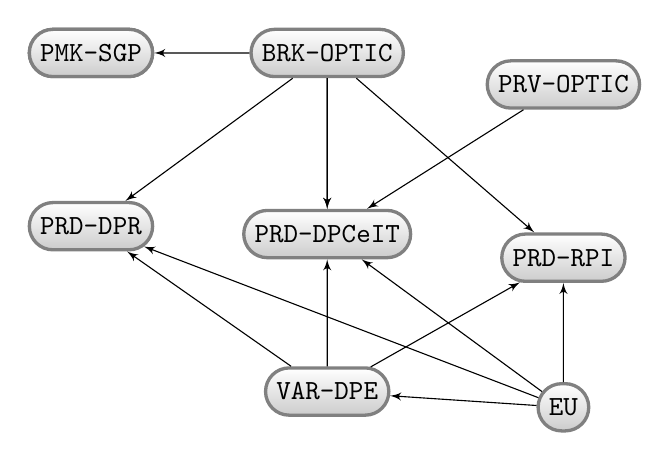
\begin{tikzpicture}[node distance=5mm]
\node [terminal] (sgp) {PMK-SGP};
\node [terminal, right of=sgp,xshift= 15mm, node distance=1.5cm] (optic) {BRK-OPTIC};
\node [terminal, right of=optic,xshift= 15mm, yshift= -4mm, node distance=1.5cm] (opticprv) {PRV-OPTIC};
\node [terminal, below of=sgp, yshift= -7mm, node distance=1.5cm] (dpr) {PRD-DPR};
\node [terminal, below of=optic, yshift= -8mm, node distance=1.5cm] (dpc) {PRD-DPCeIT};
\node [terminal, below of=opticprv, yshift= -7mm, node distance=1.5cm] (rpi) {PRD-RPI};
\node [terminal, below of=dpc, yshift= -5mm, node distance=1.5cm] (var) {VAR-DPE};
\node [terminal, below of=rpi, yshift= -4mm, node distance=1.5cm] (eu) {EU};
% Draw edges
\path [line] (optic) -- (sgp);
\path [line] (optic) -- (dpr);
\path [line] (optic) -- (dpc);
\path [line] (optic) -- (rpi);
\path [line] (opticprv) -- (dpc);
%% \path [line] (spg) -- (dpr);
%% \path [line] (spg) -- (rpi);
%% \path [line] (spg) -- (dpc);
%% \path [line] (spg) -- (var);
\path [line] (eu) -- (dpc);
\path [line] (eu) -- (dpr);
\path [line] (eu) -- (rpi);
\path [line] (eu) -- (var);
\path [line] (var) -- (dpc);
\path [line] (var) -- (dpr);
\path [line] (var) -- (rpi);
\path [line] (optic) -- (dpc);
\node [terminal] (sgp) {PMK-SGP};

   \end{tikzpicture}
\caption{Interactions between SDI Stakeholders}
\label{fig5}
\end{center}
\end{figure}


\subsubsection{ADMINISTRATIVE INTEROP.}
Perhaps the administrative interoperability, and even semantics, are the two areas in which progress has been less in terms of definition of SDI. The update of geographic data is a costly task. The SDIs facilitate the information to be provided and administered by the authentic sources of information, and  the geographic dataset from each source to be used and analyzed collaboratively. In this respect  the SDIs have facilitated the avoidance of costs  duplication  in time and effort, since it is not necessary  to duplicate  the information.
However most SDI require more detailed analysis regarding the quality of the generated data, the overlapping  information when the competences of the sources are not clear, and the use and interpretation of information. This topology of interoperability requires an exhaustive work,  a macro and collaborative analysis, as well as an agreement of the data flow and structure from larger scales.


\subsubsection{SEMANTIC INTEROP.}
While an SDI requires agreement on which technologies are applied in communication and collaborative work in relation to the management of one space, and an analysis of the associated business processes, also needs to agree on which data and metadata are exchanged. Delgado Fern\' andez et al. in \cite{Delgado} describe how the SDIs benefit from the common use of ontologies. 



\subsection{DC IN SDI}

Spatial data sharing and analysis requires a change in the SDI stakeholders think about themselves and a change of how they think the space. With SDI, spatial knowledge is a consecuence of a shared
coproduction of the space by many actors (land management sectors such as planners, geologists, forester, etc.) so the stakeholders should not be working in isolation but in social networks. SDI introduces a change
in the identity of the organization. It does not change its organizational goals but in the way its get them
working collaboratively with the help of more capable others.

Besides, SDI introduces epistomological, hermeneutical, cognitive and sociological issues. The fact that the space knowledge is structured differently as an organization does working isolated, introduce epistemological changes. The fact that SDI stakeholders should apply a shared representation of the space' knowledge imply to a apply a common interpretation. Distributed cognition behind SDI involves also interpretation of spatial data which is the product of collective negotiation. 


What encourage the sense of belonging to spatial communities \cite{Noucher2}, as well as what facilitate and hinder the attribution of common meaning to data \cite{Noucher1} are cognitive and sociological issues. 
SDI unveils shared meaning \cite{Noucher1}, materializing the geographical interactions needed to work in colaboration, and which are inherent of a common representation of the space. 
These new technological objects, are product of reification of the social interaction (according to Durkheim \cite{Durkheim} we should consider social facts as things), but needed to be appropiately defined, due to the fact they are product of the knowledge engeneering and sostained cognitive activities from several organizations. 

% So, they stress the importance of the contribution of knowdledge theories. 
During data appropiation process Noucher et al. \cite{Noucher1} identify two different dialectic process  performed by stakeholders of land management: Individual projection and collective negotiation.
The former is based on expectation and experience of the stakeholder. The latter is based on participation
and reification process. 


\Section{CONCLUSIONS}

Technologies are usually mediators instruments of society helping to its members to interact and interchange in performing their goals. With the introduction of web technologies 2.0 and 3.0, applications are built  of a network of cooperating data services and users are important value added of their own data to those provided by the application, the emphasis of the application is focused on the coordination and interactions. 
When technology is used as an instrument by communities of practice, or even by a more wider set of organizations, harmonization and orquestation of services are required, members' roles and interoperability should be analized. 
These technological changes, demands profound cultural investments in members and organizations due to the fact that data is a shared resource and object of interchange, relationships and interactions are materialized vehicles in social networks with specific roles. This flow and interaction should be analized from cognitive theories. The investment of efforts (in time and cost) are profitable, the analysis of aspects of cognition in distributed communities of practice allow substantial improvements in how knowledge is perceived, retrieved, transfered and applied (cognitive improvements).

%%!!!!Inherently, there exists many social factors contributing to cognitive development. 

We believe that societies facing such crucial changes of its process traverse important cognitive changes: knowledge is organized in a different way (introducing epistemological changes), and by consequence, this impacts in the way the society interpret the information it should deal (hermeneutic aspects that should also be considered). Our razoning is that: distributed cognition (which enhances the understanding of interactions between humans, machines and environments) within communities of practice around web applications provides a suitable context to analyze the aforementioned problematic. Based on a set of interviews and the experience related to our case of study, spatial data infraestructure, we understand cognitive issues inside these communities. Data armonization and services orquestations requered by these changes, also contributes to their sense of identity and improve its capacity of agency proxy. Community interoperability (ability of making systems and organizations to work together) plays a central role in the process of 'making meaning',
being perception of process information (issue of cognition) influenced by sense and meaning. 

%Social interaction in the development of cognition (Vygotsky) plays an important role in the process of 'making meaning'.
%Distributed cognition illustrates the process of interaction between people and technologies in order to determine how to best represent, store and provide access to digital resources and other artifacts.

%What distinguishes distributed cognition ....from other approaches also concerns to the boundaries of the unit of analysis for cognition.

As a future work we intend to continue to deepen the qualitative analysis of cognitive aspects that occur in these types of technological assemblies in society, applying methodologies of grounded theory which can guide us in a theoretical samply of data. We also plan to apply focus group techniques within communities of practice.

%\vspace{0.2cm}

\noindent {\bf ACKNOWLEDGMENTS}

\noindent This research is part of the 048/12 'Hacia el Fortale- cimiento de la Sociedad en el Uso y Aplicaci\' on Geoespacial y las TICS' of Patagonia San Juan Bosco University and the 'Modelos y Tecnolog\' {\i}as para Gobierno Electr\' onico' of Comahue University (Argentina).

\bibliographystyle{ieeetr}
\bibliography{latex8}

\end{document}

